% Netzwerkanltung für die Studentenstadt Freimann
% Tex initially created by Maximilian Engelhardt <maximilian.engelhardt@stusta.mhn.de>

%\documentclass[a4paper,12pt,draft]{scrartcl}
\documentclass[a4paper,12pt]{scrartcl}

\usepackage[utf8]{inputenc}
\usepackage{eurosym}
\usepackage{tabularx}
\usepackage[pdftex,final]{graphicx}
\usepackage{wrapfig}
\usepackage[top=1.5cm,bottom=2.5cm,left=1.5cm,right=1.5cm]{geometry}
%\usepackage[margin=2cm]{geometry}
\usepackage{hyperref}
% For emphasizing the names of options, buttons, tabs, etc. which should be set apart from the rest of the text
\newcommand{\optemph}[1]{\textbf{#1}}


\title{Student residence Max-Bill:\\
       Internet configuration guide}
\date{\today}

\begin{document}

\maketitle

\begin{figure}[t!]
   \centering
   \vspace{-20pt}
   
\includegraphics[width=0.8\textwidth,keepaspectratio]{Bilder/StuStaNet_Logo}
   \vspace{-20pt}
\end{figure}

\section*{General information about your Internet connection}

This set-up guide will help you to configure your computer to access the Max-Bill network as well as the Internet. Before attempting to connect to the Internet please read the terms of use, which can be found at the end of your housing contract.

To access the Internet you will require a computer with an ethernet connector (most computers have this feature built-in). Additionally, you will need a network cable (RJ-45 patch cable) to connect your computer to the network outlet located on the wall of your room. Should you not have a network cable, you can purchase a cable from the StuStaNet. See below for more information

You are responsible for your computer's network activity. You must ensure that it does not pose a threat to any other computer on the network and that it is secured and protected from possible virus- and malware infection. This involves:
\begin{itemize}
    \item Keeping your computer updated with the latest security updates
    \item Updating your anti-virus program regularly
    \item Using a personal firewall
\end{itemize}
If the StuSta detects that your computer is infected by a virus and poses a threat to the computer network, your Internet connection will be cut off.

\begin{em}
In case of repeated infractions, your Internet connection will be permanently terminated.
\end{em}

These drastic measures are necessary because the entire network can be crippled by a single infected computer. Furthermore, the Leibniz Supercomputing Centre (Leibniz-Rechenzentrum, LRZ), which provides the Max-Bill residence with Internet access, will block all Internet traffic from the entire residence if they detect a computer virus.

\emph{Please note:} If you are a beginner and don't have the technical know-how necessary to keep a Windows system secure, the StuStaNet recommends that you consider installing a GNU/Linux operating system such as Ubuntu. You can download Ubuntu at \url{http://www.ubuntu.com}.


\section*{Membership in the StuStaNet~e.V.}

Membership in the StuStaNet~e.V. requires a one-time fee of \EUR{20} and has a number of advantages including (in addition to Internet via Proxy), full Internet over a NAT masquerader, your own e-mail address, webspace with PHP and database support\footnote{\url{http://stusta-wiki.de/Services}}.

You can join the StuStaNet~e.V. at one of our network administrators at Max-Bill or at our office hours, which are Mondays and Thursdays from 19.00 to 19.30 in the Blue House (House \#11) of Studentenstadt, room 0028, during the semester (during breaks only Thursdays).

If you are interested in our network and our servers or if you would just like to contribute some ideas, you can become a network administrator (elections are at the beginning of each semester in each house) or just visit our monthly meeting (Adminrat). This meeting takes place on the first Thursday of every month at 20.00 in the Hackerspace\footnote{2nd floor, House 10, Hans-Leipelt-Str. 7}. Although the meetings are usually held in German, we can certainly make accommodations for non-German speakers.

\section*{More Information}

If you are experiencing problems please consult the Stusta-Wiki and the Info-Site:

\begin{center}
  \begin{tabularx}{\linewidth}{|lX|}
    \hline
    \url{http://stusta-wiki.de/Main_Page} & Network help, information about living in the Studentenstadt, Shopping in the area, Doctors, Nightlife\dots\\
    \hline
    \url{http://info.stusta.mhn.de/} & Announcements and general information about the StuSta. Unfortunately, there's no English version yet.\\
    \hline
  \end{tabularx}
\end{center}
Should you experience problems configuring your Internet access, you can contact a network administrator. A list of network administrators is on display on the ground floor of your house.

Keep in mind that the administrators are only responsible for network-related problems, i.e. problems directly involving your connection to the Internet and other computers in the StuStaNet.

\newpage
\section*{Tips on securing your computer}

Here are a few tips on securing your computer against harmful software.

\subsection*{Anti virus programs}
\paragraph*{Windows}
\begin{center}
  \begin{tabularx}{\linewidth}{|p{.2\linewidth}XX|}
    \hline
    Name & Website & Description\\
    \hline \hline
    Avira AntiVir & \url{http://www.free-av.com/} & free, since 1988\\
    \hline
    Microsoft Security Essentials & \url{http://www.microsoft.com/security\_essentials/} & free, by Microsoft, also anti spyware\\
    \hline
    Sophos Antivirus & \url{http://sophos.lrz-muenchen.de/} & Commercial software which is supplied by the LRZ, that can be used for free by students\\
    \hline
    avast! & \url{http://www.avast.com/} & Home Edition free for private use\\
    \hline
  \end{tabularx}
\end{center}

There are numerous other anti-virus programs such as Kaspersky, Norton and McAffee. However, these programs are commercial and require a paid license.

\paragraph*{MacOS (Apple)}
\begin{center}
  \begin{tabularx}{\linewidth}{|p{.2\linewidth}XX|}
    \hline
    Name & Website & Description\\
    \hline \hline
    Avira Free Mac Security & \url{https://www.avira.com/en/avira-free-mac-security} & free\\
    \hline
    Sophos Antivirus & \url{http://sophos.lrz-muenchen.de/} & Commercial software which is supplied by the LRZ, that can be used for free by students\\
    \hline
    avast! Free AV for MAC & \url{http://www.avast.com/free-antivirus-mac} & Free Edition free for private use\\
    \hline
  \end{tabularx}
\end{center}

There are numerous other anti-virus programs such as Kaspersky, Norton and Bitdefender. However, these programs are commercial and require a paid license.

\paragraph*{Linux}

There is no need to use an anti virus package with this operating system. Due to its small market share and different software architecture, this platform is mostly virus-free (for now). There are still programs available to prevent your computer from spreading Windows viruses; the programs listed above may have such versions for Linux.

\pagebreak

\subsection*{Anti-spyware Programs}

Spyware is used to spy on users and to collect personal information. You can find more information on Wikipedia\footnote{\url{http://en.wikipedia.org/wiki/Spyware}}.

\begin{center}
  \begin{tabularx}{\linewidth}{|p{.18\linewidth}Xp{.3\linewidth}|}
    \hline
    Name & Website & Description\\
    \hline \hline
    Windows Defender & \url{http://www.microsoft.com/en-us/download/details.aspx?id=17} & Integrated in Microsoft Security Essentials\\
    \hline
    Spybot, Search \& Destroy & \url{http://www.safer-networking.org/} & Free for private use\\
    \hline
    Ad-Aware & \url{http://www.lavasoft.com/products/select\_your\_product.php} & Free version available\\
    \hline
  \end{tabularx}
\end{center}

There are numerous other anti-spyware programs, most of which are commercial software. These usually come in combination with a firewall or anti virus program.

\subsection*{Personal Firewalls}

A firewall controls the connection between a computer and the network to which the computer is connected. You can find more information on Wikipedia\footnote{\url{http://en.wikipedia.org/wiki/Personal\_Firewall}}.

Almost every anti-virus program, and even some anti-spyware software, has an integrated firewall .

In general, the integrated firewall of an operating system is not sufficient to ensure complete protection.
\newpage

\section*{Network configuration}

Each network outlet is assigned eight IP addresses and the IP range is marked on the outlets. Also you should have received a note containing your networksettings with your rental agreement. If you did not get the note containing the networksettings, please refer to the administration.

\subsection*{Overview}

To successfully connect to the Internet you need to follow these steps:
\begin{itemize}
    \item Connect to the network outlet (Ethernet jack)
    \item Configure the network settings in your operating system
    \item Enter proxy information~/ proxy script into your Web browser
\end{itemize}


\begin{center}
  \begin{tabularx}{\linewidth}{|lXp{.2\linewidth}|}
    \hline
    Setting & Value & Example \\
    \hline \hline
    IP address & \nolinkurl{10.149.xxx.yyy} - \nolinkurl{10.149.xxx.zzz}, \newline 8 addresses are available which are marked on the network point & \nolinkurl{10.149.243.16} - \nolinkurl{10.149.243.23} \\
    \hline
    Subnet mask & \nolinkurl{255.255.255.0} & \\
    \hline
    Standard gateway & \nolinkurl{10.149.xxx.254} \newline first three blocks like the IP address, fourth block \nolinkurl{254} & \nolinkurl{10.149.243.254} \\
    \hline
    DNS server (Nameserver) & \nolinkurl{10.149.8.2} & \\
    \hline
    DNS suffix (Domainname) & \nolinkurl{stusta.mhn.de} & \\
    \hline
    Proxy script & \multicolumn{2}{l|}{\nolinkurl{http://wpad.mb67.stusta.mhn.de/proxy.pac}} \\
    \hline
    Proxy server (manual) & \multicolumn{2}{l|}{\nolinkurl{http://proxy.mb67.stusta.mhn.de:3128}} \\
    \hline
  \end{tabularx}
\end{center}

You must use either the proxy script (preferred) or the manual proxy configuration.

\subsection*{Connection to the network outlet}

You should only use the left Ethernet socket.

\emph{Attention}: It is \emph{prohibited} to connect a telephone, ISDN equipment or any similar devices to the left network connection point as these cause massive network disruptions in the Sudentenstadt and can cause damage to our network hardware.

\subsection*{E-mail, Skype, ICQ, Online games, ...}

The Internet connection in the Sudentenstadt is intended for academic and scientific purposes only.

The standard Internet access in the Max-Bill residence is limited to browsing only (Connections via the HTTP proxy) as well as internal connections to the Munich Scientific Network (Münchner Wissenschaftsnetz, MWN). Sending e-mail over POP3~/ IMAP, using instant messaging and playing online games is only possible with a StuStaNet~e.V. membership (see above).

\subsection*{Wifi in StuSta}
There is no central wifi in StuSta, due to massive concrete walls.

But you can setup your own wifi. If you do so, please consinder this:
\begin{itemize}
    \item Proper country selection (DE)
    \item Only use Channels 1, 6 or 11 or use 5 GHz
    \item Use secure encryption and passwords (WPA2 only)
\end{itemize}

If you use an AccessPoint (AP), every device connected needs one of the eight room IPs assigned manually. If you use a wifi-router, it need one of the room IPs assigned (and all the other configuration as described before, like netmask and gateway). The router will then configure connected devices automaticaly, providing it is configured properly. (Non-members have to configure the Proxy in all cases on every single device connected.)

\vspace{2em}

StuStaNet e. V. sells pre-configured and easy to setup wifi-routers during office ours (members only).

\newpage

\begin{figure}[t!]
    \raggedleft
    \vspace{-20pt}
    
\includegraphics[height=1cm,keepaspectratio]{Bilder/Ubuntu_logo}
    \vspace{-30pt}
\end{figure}

\section*{Step by step instructions}
\subsection*{Ubuntu settings}
\begin{enumerate}
	\item Open the network configuration dialog by clicking on \optemph{System} $\rightarrow$ \optemph{Settings} $\rightarrow$ \optemph{Network Settings}.
	\item Select your network card in the first tab (normally eth0) and click on \optemph{Edit}.
	\item Click on the IPv4-Settings tab and change the method to \optemph{Manually}.
	\item Under \optemph{Addresses} click on Add.
      \begin{figure}[h!]
        \centering
        \begin{minipage}[c]{0.45\linewidth}
          \centering
          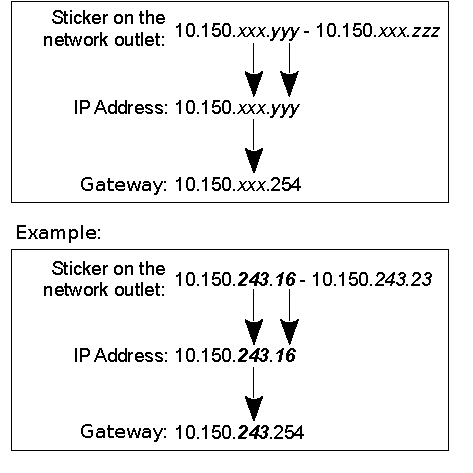
\includegraphics[width=\linewidth,keepaspectratio]{Bilder/IP_Gerneric_EN}
        \end{minipage}
        \begin{minipage}[c]{0.5\linewidth}
          \centering
          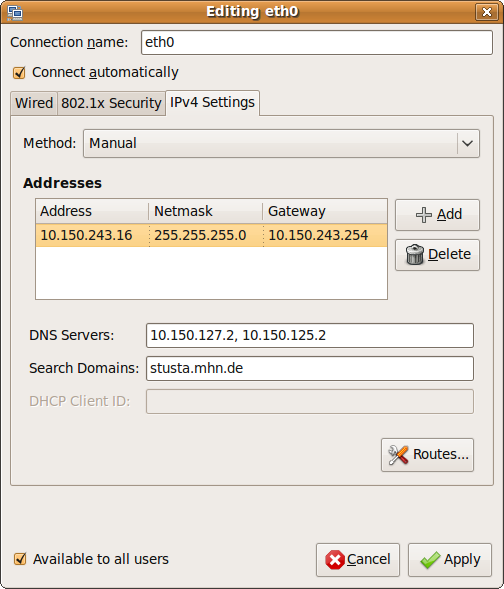
\includegraphics[width=\linewidth,keepaspectratio]{Bilder/IP_Ubuntu_EN}
          \caption{Example network configuration in Ubuntu Linux}
          \vspace{-15pt}
        \end{minipage}
      \end{figure}
  \item Now enter the IP address, the subnet mask, the gateway, the DNS and the search domain. The DNS server addresses are \nolinkurl{10.149.8.2}, the search domain is \nolinkurl{stusta.mhn.de} and the subnet mask is \nolinkurl{255.255.255.0}. You can find your IP address on the note containing your networksettings which you received with your rental agreement. If you did not get the note containing the networksettings, please refer to the administration. Confirm the settings with \optemph{OK} and close the window.
\end{enumerate}
\vspace{-15pt}
\paragraph*{Global proxy settings}
You can define a global proxy server in Ubuntu so that you don't have to configure it for each browser individually.
\begin{enumerate}
	\item Open the network proxy settings by clicking on \optemph{System} $\rightarrow$ \optemph{Settings} $\rightarrow$ \optemph{Network Proxy}.
    \item At the bottom of the window, mark the automatic proxy configuration box and enter the auto-configuration URL: \url{http://wpad.stusta.mhn.de/proxy.pac}\ . Close the window to save the settings.
\end{enumerate}
$\rightarrow$ Your Internet access is now configured.



\newpage
\enlargethispage{20pt}

\begin{figure}[t!]
    \raggedleft
    \vspace{-20pt}
    
\includegraphics[height=1cm,keepaspectratio]{Bilder/Windows_logo}
    \vspace{-20pt}
\end{figure}

\section*{Step by step instructions}
\subsection*{Windows settings}
\paragraph*{Windows XP}
\begin{enumerate}
	\item Open Control Panel by clicking on \optemph{Start} $\rightarrow$ \optemph{Control Panel}.
    \item Click on \optemph{Network and Internet Connections}.
	\item Click on \optemph{Network Connections}.
	\item Right click on the \optemph{Local Area Connection} and select \optemph{Properties}.
\end{enumerate}
$\rightarrow$ Continue at point 5.
\paragraph*{Windows Vista/7}
\begin{enumerate}
	\item Open Control Panel by clicking on \optemph{Start} $\rightarrow$ \optemph{Control Panel}.
    \item Click on \optemph{Network and Internet} then on \optemph{View network status and tasks}.
	\item Click on \optemph{Change adapter settings} and then right click on the \optemph{Local Area Connection} and select \optemph{Properties}.
\end{enumerate}
$\rightarrow$ Continue at point 5.
      \begin{figure}[h!]
	\centering
        \vspace{-5pt}
        \begin{minipage}[c]{0.45\linewidth}
          \centering
          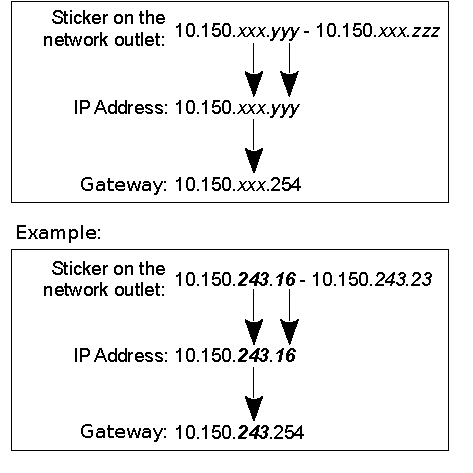
\includegraphics[width=\linewidth,keepaspectratio]{Bilder/IP_Gerneric_EN}
        \end{minipage}
        \begin{minipage}[c]{0.48\linewidth}
          \centering
          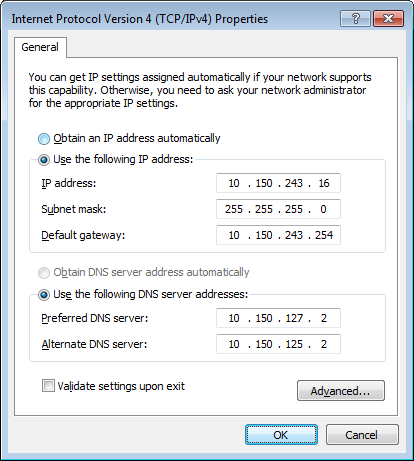
\includegraphics[width=\linewidth,keepaspectratio]{Bilder/IP_Windows_EN}
          \caption{Example network configuration in Windows Vista}
        \end{minipage}
      \vspace{-15pt}
      \end{figure}
\paragraph*{Windows 8}
\begin{enumerate}	
	\item To open Control Panel press the Windows-Key and type Control Panel, then press ENTER.
    \item Click on \optemph{Network and Internet} then on \optemph{View network status and tasks}.
	\item Click on \optemph{Change adapter settings} and then right click on the \optemph{Local Area Connection} and select \optemph{Properties}.
\end{enumerate}
$\rightarrow$ Continue at point 5.
\paragraph*{Windows XP/Vista/7/8}
\begin{enumerate}
    \setcounter{enumi}{4}
	\item Select \optemph{Internet Protocol Verson 4 (TCP/IPv4)} (Windows Vista)/ \optemph{Internet Protocol  (TCP/IP)} (Windows XP) and click on \optemph{Properties}.
    \item Now type in the IP address, the subnet mask, the Default gateway and the DNS Server. The DNS Server addresses are \nolinkurl{10.149.8.2}, the Subnet mask is \nolinkurl{255.255.255.0}. You can find your IP address on the note containing your networksettings which you received with your rental agreement. If you did not get the note containing the networksettings, please refer to the administration.
    \item Click on Advanced and click on the DNS tab. Type \nolinkurl{stusta.mhn.de} in the DNS suffix for this connection field.
	\item Confirm the settings with \optemph{OK} and close the window.
\end{enumerate}
$\rightarrow$ Continue with the browser settings.



\newpage

\begin{figure}[t!]
    \raggedleft
    \vspace{-20pt}
    
\includegraphics[height=1cm,keepaspectratio]{Bilder/OSXLeopard}
    \vspace{-20pt}
\end{figure}

\section*{Step by step instructions}
\subsection*{Mac OS X settings}
\begin{enumerate}
	\item Click on the \optemph{Apple logo} (top left) and select \optemph{System Preferences} $\rightarrow$ \optemph{Network}.
	\item Select the \optemph{Ethernet} connection.
	\item Set the \optemph{Configure IPv4} drop-down box to \optemph{Manually}.
	\item Now type in the IP address, the subnet mask, the gateway, the DNS and the search domain. The DNS server addresses are \nolinkurl{10.149.8.2}, the search domain is \nolinkurl{stusta.mhn.de} and the subnet mask is \nolinkurl{255.255.255.0}. You can find your IP address on the note containing your networksettings which you received with your rental agreement. If you did not get the note containing the networksettings, please refer to the administration. Confirm the settings with \optemph{Apply}.
      \begin{figure}[h!]
      \centering
%      \vspace{-5pt}
        \begin{minipage}[c]{0.38\linewidth}
          \centering
          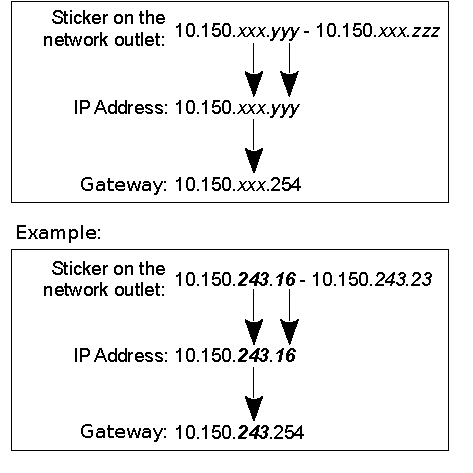
\includegraphics[width=\linewidth,keepaspectratio]{Bilder/IP_Gerneric_EN}
        \end{minipage}
        \begin{minipage}[c]{0.60\linewidth}
          \centering
          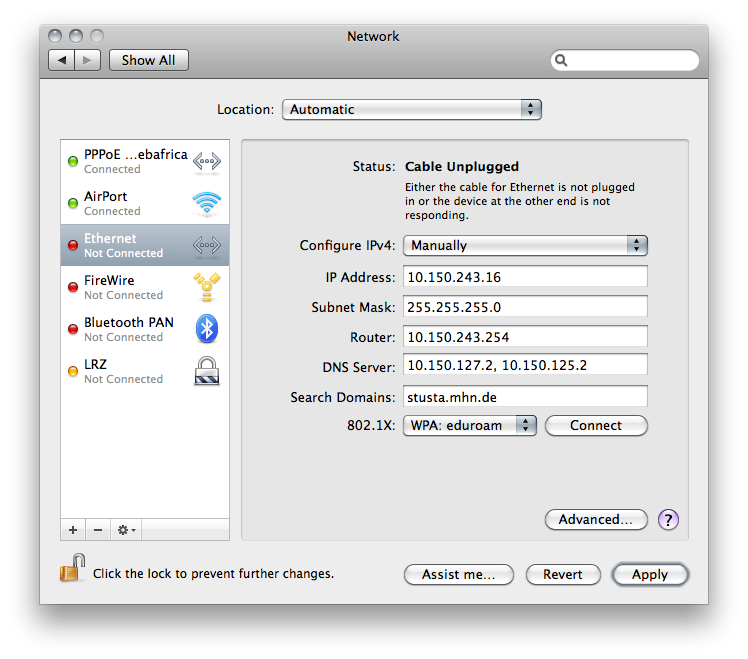
\includegraphics[width=\linewidth,keepaspectratio]{Bilder/IP_Mac_EN}
          \caption{Example network configuration in Mac OS X}
        \end{minipage}
%      \vspace{-15pt}
      \end{figure}
\end{enumerate}

\paragraph*{Global proxy settings}
You can define a global proxy server in Mac OS X so that you don't have to configure it for each browser individually. Firefox, however, still needs an individual configuration (see Browser settings)
%\begin{wrapfigure}{r}{0.4\textwidth}
%  \vspace{-20pt}
%  \begin{center}
%    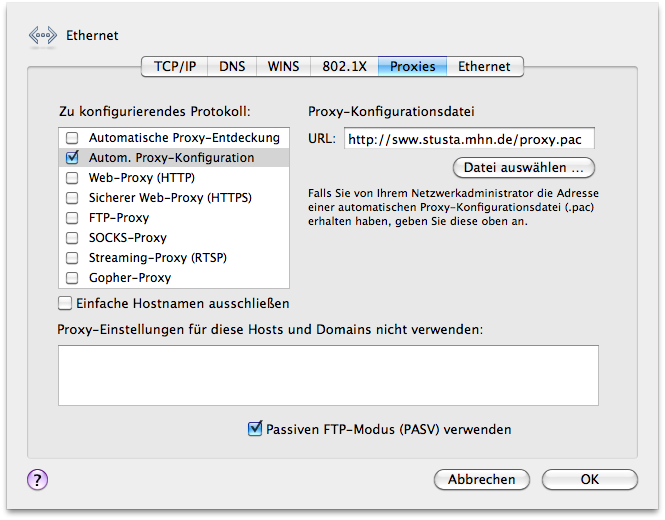
\includegraphics[width=0.48\textwidth,keepaspectratio]{Bilder/Proxy_MAC}
%  \end{center}
%  \vspace{-20pt}
%  \caption{Beispielhafte Proxyeinstellungen unter Mac OS~X}
%  \vspace{-10pt}
%\end{wrapfigure}
\begin{enumerate}
	\item Click on \optemph{Advanced} and select the \optemph{Proxies} tab
	\item Mark the checkbox next to \optemph{Automatic Proxy Configuration} and type in the URL \url{http://wpad.mb67.stusta.mhn.de/proxy.pac}\ . Click on \optemph{OK} and select \optemph{Apply} one more time. You can now close System Preferences.
\end{enumerate}
$\rightarrow$ Your Internet access is now configured.

\newpage

\section*{Browser settings}

\begin{wrapfigure}{r}{0.5\textwidth}
  \vspace{-30pt}
  \begin{center}
    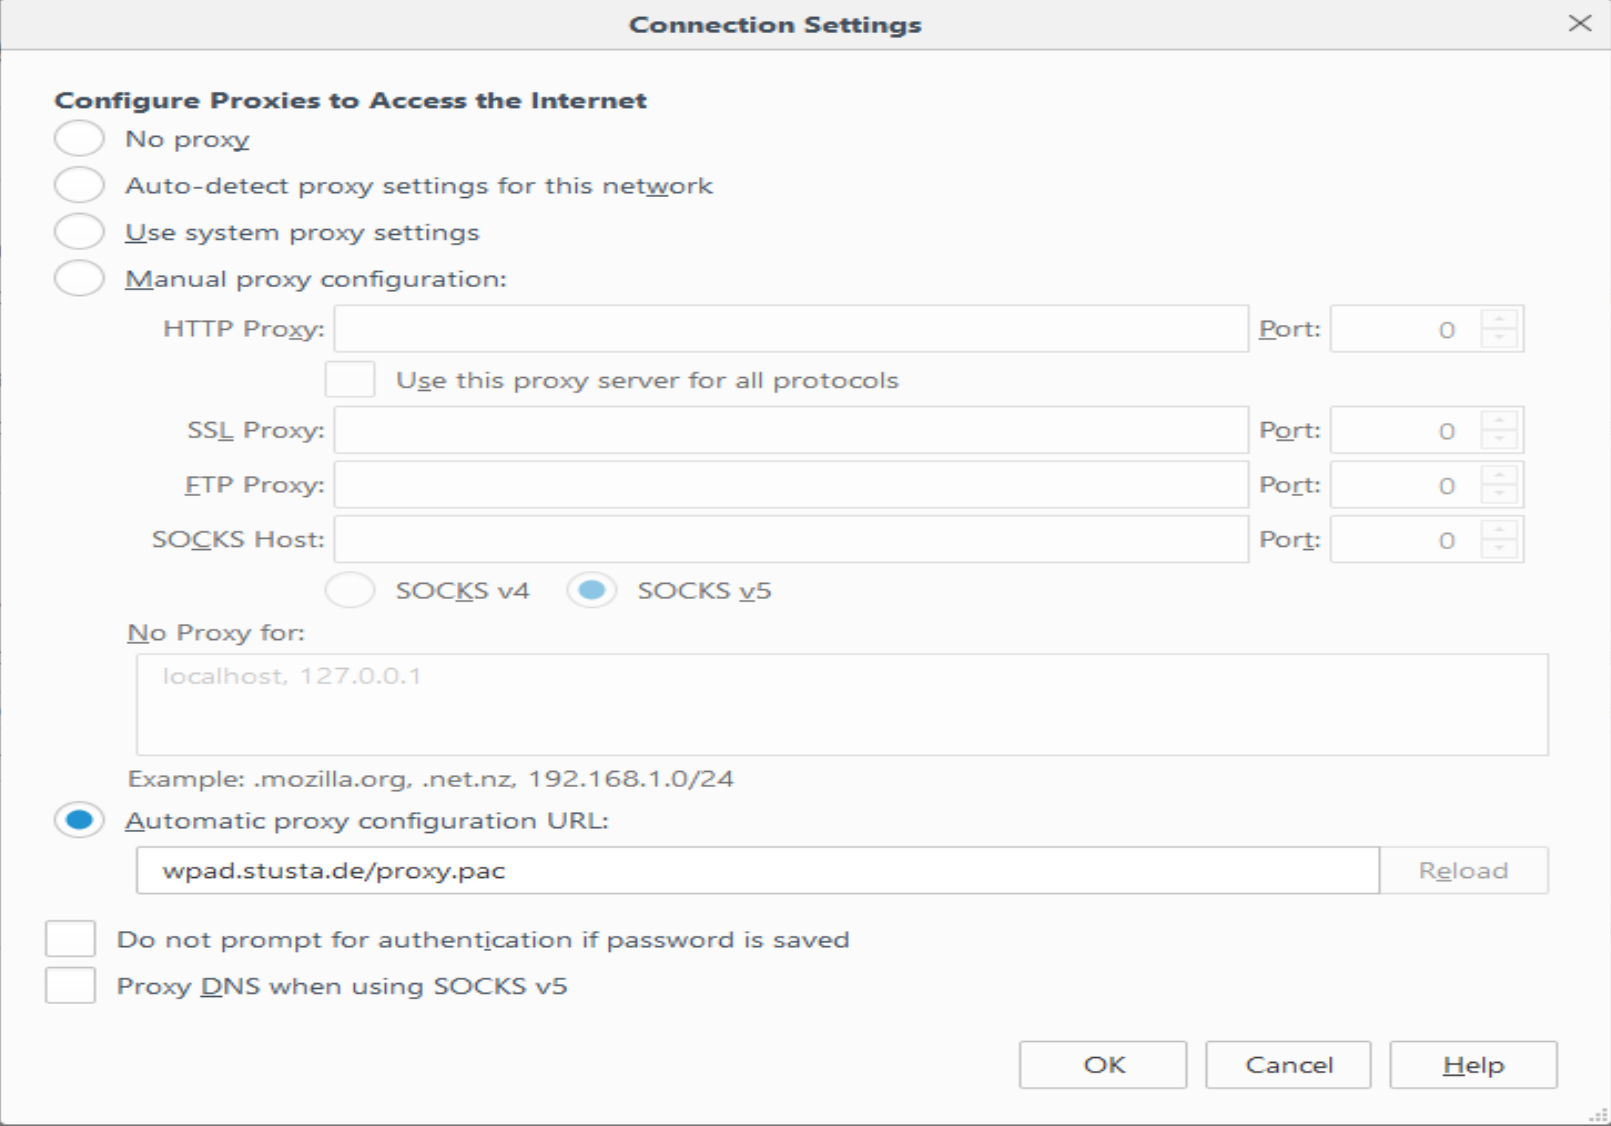
\includegraphics[width=0.5\textwidth,keepaspectratio]{Bilder/Proxy_Firefox_EN}
  \end{center}
%  \vspace{-20pt}
  \caption{Configuring the proxy script in Mozilla Firefox}
%  \vspace{-10pt}
\end{wrapfigure}

\subsection*{
\includegraphics[height=1.2cm,keepaspectratio]{Bilder/Firefox_35_logo} Mozilla Firefox}
\begin{enumerate}
    \item Start Firefox.
	\item Click on \optemph{Edit} $\rightarrow$ \optemph{Preferences}.
	\item Click on \optemph{Advanced} and select the \optemph{Network} tab.
	\item Click on \optemph{Settings}.
    \item Select the bottommost option and use \\ \url{http://wpad.mb67.stusta.mhn.de/proxy.pac} as the Automatic proxy configuration URL.
	\item Confirm with \optemph{OK} and close the remaining windows.
\end{enumerate}
$\rightarrow$ Your Internet access is now configured.


\begin{wrapfigure}{r}{0.5\textwidth}
%  \vspace{-20pt}
  \begin{center}
    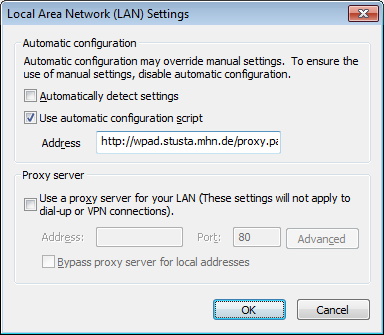
\includegraphics[width=0.5\textwidth,keepaspectratio]{Bilder/Proxy_IE_EN}
  \end{center}
%  \vspace{-20pt}
  \caption{Configuring the proxy script in Internet Explorer}
%  \vspace{-10pt}
\end{wrapfigure}

\subsection*{
\includegraphics[height=1.2cm,keepaspectratio]{Bilder/Internet_Explorer_7_Logo} Internet Explorer}
\begin{enumerate}
    \item Start Internet Explorer.
	\item Click on \optemph{Tools} and select \optemph{Internet Options}.
	\item In the \optemph{Connections} tab, select the \optemph{LAN Settings} button.
	\item Mark the \optemph{Use automatic configuration script} checkbox and type in the URL: \\ \url{http://wpad.stusta.mhn.de/proxy.pac}
	\item Confirm with \optemph{OK} and close the remaining windows.
\end{enumerate}
$\rightarrow$ Your Internet access is now configured.

\newpage
\begin{wrapfigure}{r}{0.5\textwidth}
%  \vspace{-20pt}
  \begin{center}
    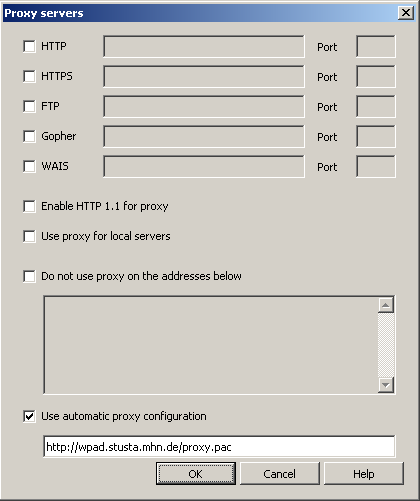
\includegraphics[width=0.5\textwidth,keepaspectratio]{Bilder/Proxy_Opera_EN}
  \end{center}
%  \vspace{-20pt}
  \caption{Configuring the proxy script in Opera}
%  \vspace{-10pt}
\end{wrapfigure}

\subsection*{
\includegraphics[height=1.2cm,keepaspectratio]{Bilder/Opera_O} Opera}
\begin{enumerate}
    \item Start Opera.
	\item Click on \optemph{Tools} and select \optemph{Settings} $\rightarrow$ \optemph{Preferences}.
	\item Click on the \optemph{Advanced} tab, select the \optemph{Network} category on the left and click on the \optemph{Proxy servers} button.
	\item Mark the \optemph{Use automatic proxy configuration script} checkbox and type in this URL: \\ \url{http://wpad.stusta.mhn.de/proxy.pac}
    \item Close both windows by clicking on OK.
\end{enumerate}
$\rightarrow$ Your Internet access is now configured.


\end{document}
